\documentclass[10pt,conference]{IEEEtran}

\usepackage{amsmath,amssymb,amsfonts}
\usepackage{graphicx}
\usepackage{booktabs}
\usepackage{textcomp}
\usepackage{xcolor}
\usepackage{tikz}
\usetikzlibrary{arrows.meta,positioning}
\usepackage{cite}
\usepackage{hyperref}

\def\BibTeX{{\rm B\kern-.05em{\sc i\kern-.025em b}\kern-.08em
    T\kern-.1667em\lower.7ex\hbox{E}\kern-.125emX}}

\begin{document}

\title{Cooperative Vision-Based Localization and MPC Formation Control\\ for a LIMO Robot Swarm Tracking a Moving Person}

\author{
\IEEEauthorblockN{Marco Misseroni, Federico Battisti}
\IEEEauthorblockA{MSc Mechatronics Engineering -- Electronics and Robotics\\
University of Trento\\
Intelligent Distributed Systems course project}
}

\maketitle

\begin{abstract}
We present the implementation, on a real three-robot LIMO fleet, of a fully distributed
cooperative tracking system in which each robot fuses wheel odometry with ArUco-based relative
observations of its teammates and of a tracked person, using a decentralized recursive filter
that reconstructs, on demand and without ever broadcasting a full joint covariance matrix, the
same estimate a centralized Extended Kalman Filter would produce. Each robot combines this
locally-consistent pose estimate with a Model Predictive Controller that drives it into one of
three slots of a rigid formation orbiting the person, the slot assignment being solved locally
by every robot as a linear assignment problem so that no single node coordinates the team. Unlike
a purely simulated study, this work is constrained by an actual ROS~2 software stack running on
three physical differential-drive robots communicating over a shared network, and we report
results from logged on-robot data rather than from a large synthetic parameter sweep. We discuss
the architecture end to end -- perception, estimation, formation planning, and control -- analyze
the covariance behaviour of the cooperative filter on a real run, including its sensitivity to
the initial covariance of an agent with no self-motion sensing, and catalogue the concrete
implementation issues (a silent formation-controller bug, dead topics, and README/code
divergences) that surfaced only once the system had to run outside simulation.
\end{abstract}

\section{Introduction}

Coordinating a team of mobile robots to keep a moving person inside a stable, useful geometric
formation is a recurring building block of assistive and surveillance robotics: an escort of
robots can carry sensors, lighting, or communication relays around a person while none of them
occupies a privileged, failure-prone ``leader'' role. The goal of this project is to build and
run, on real hardware, such a system: three LIMO differential-drive robots that (i) perceive each
other and a person carrying a fiducial marker through their onboard cameras, (ii) fuse those
relative observations with their own odometry into a locally-consistent pose estimate of the
whole team without any of them ever seeing the others' full state, and (iii) use that estimate to
drive into and hold a triangular formation around the person as it moves, entirely through
peer-to-peer ROS~2 communication and without a central coordinator.

The estimation core is an implementation of Interim Master Decentralized Cooperative Localization
(IMDCL) \cite{kia2016}, which lets every agent recover the cross-covariance terms a centralized
filter would carry, using only pairwise messages exchanged at the moment a relative measurement
occurs. Perception is vision-only: ArUco markers \cite{aruco2014} mounted on the three robots and
on the person substitute for the pretrained human detector the project was originally scoped
around. Formation-keeping is delegated to a finite-horizon MPC solved with CasADi/IPOPT
\cite{casadi2019,wachter2006}, with the desired slot for each robot chosen through a Hungarian
assignment \cite{kuhn1955} that every robot solves independently on its own local copy of the
team's state.

Framing this work against a companion project in the same course
\cite{renelli-zanolini-artva}, which develops a comparably distributed multi-drone estimator over
a 12420-run simulated sweep across synthetic alpine terrain, is useful mainly to state the
difference in kind: that work is a statistical characterization of an algorithm across a designed
parameter space, while this one is a single software/hardware stack that has to survive real
camera noise, real wheel odometry, and the accidents of an un-simulated ROS~2 graph.
Sec.~\ref{sec:results} is written accordingly: instead of success rates aggregated over thousands
of Monte Carlo runs, we
analyze logged covariance and correction traces from an actual run on the robots, and we report,
as part of the results, the concrete implementation defects this surfaced.

\section{Adopted Models}

\subsection{Robot and person models}

Each robot is modeled as a unicycle with state $\mathbf{x} = [x, y, \theta]^\top$ and input
$\mathbf{u} = [v, \omega]^\top$, the commanded linear and angular velocity. The filter and the
simulation model integrate it with a second-order (mid-point) discretization
(\texttt{agent\_type.py}):
\begin{align}
x_{k+1} &= x_k + \Delta t\, v_k \cos\!\left(\theta_k + \tfrac{\Delta t\, \omega_k}{2}\right) \\
y_{k+1} &= y_k + \Delta t\, v_k \sin\!\left(\theta_k + \tfrac{\Delta t\, \omega_k}{2}\right) \\
\theta_{k+1} &= \theta_k + \Delta t\, \omega_k
\end{align}
with $\Delta t = 0.1\,\mathrm{s}$, subject to the LIMO datasheet limits
$|v|\le v_{\max}=0.1477\,\mathrm{m/s}$, $|\omega|\le\omega_{\max}=0.2954\,\mathrm{rad/s}$. The
Jacobians $A=\partial f/\partial\mathbf{x}$ and $G=\partial f/\partial\boldsymbol{\eta}$ used by
the filter are the exact derivatives of this map, evaluated symbolically in
\texttt{MobileRobotModel}.

The tracked person has no actuation and no odometry of its own, so it is modeled purely as a
constant-velocity point with state $\mathbf{x}_p = [x, y, v_x, v_y]^\top$ and linear dynamics
$\mathbf{x}_{p,k+1} = A_p\,\mathbf{x}_{p,k}$,
\begin{equation}
A_p = \begin{bmatrix} 1 & 0 & \Delta t & 0 \\ 0 & 1 & 0 & \Delta t \\ 0 & 0 & 1 & 0 \\ 0 & 0 & 0 & 1 \end{bmatrix},
\end{equation}
driven only by a discretized white-noise-acceleration process covariance $Q_p$ (the standard
Van~Loan form, with the $\Delta t^4/4$, $\Delta t^3/2$, $\Delta t^2$ blocks coupling position and
velocity noise). Every correction to the person's state therefore comes exclusively from the
relative measurements the robots publish; between two such corrections its estimate simply
coasts at the last inferred velocity. This is the main structural difference from a system with
an absolute sensor (e.g. the LiDAR-altitude correction of \cite{renelli-zanolini-artva}): here
\emph{no agent has any absolute position reference at all}, robot or person alike -- the entire
team's consistency and its ability to track the person rests on the relative vision measurements
and on the cooperative bookkeeping described in Sec.~\ref{sec:localization-node}.

\subsection{Communication and measurement graph}

Two logically distinct graphs coexist. The \emph{ROS~2 communication graph} is, in practice,
complete: every one of the four estimator instances (three robots and the person, run as four
separate nodes) publishes to and subscribes from the same two mesh topics, \texttt{/info} and
\texttt{/update} (Table~\ref{tab:msgs}), regardless of camera visibility -- there is no
communication-radius model as in a radio-based fleet. The \emph{measurement graph} is instead
sparse and time-varying, exactly as in a vision-limited system: an edge $(a,b)$ exists at time
$t$ only if robot $a$'s camera currently resolves an ArUco marker belonging to agent $b$. It is
this second, sparser graph that gates when a relative correction can happen at all; the
communication mesh only decides how its effect is propagated to keep every agent's bookkeeping
consistent once it has.

\section{Solution}

The system decomposes into three cooperating subsystems that mirror the physical pipeline
sensing~$\to$~estimation~$\to$~action:

\begin{itemize}
\item \textbf{Vision} (Sec.~\ref{sec:vision-node}) turns raw camera frames into relative pose
measurements $z_{ab} = h(\mathbf{x}_b,\mathbf{x}_a) + \nu$ between an observing robot $a$ and an
observed agent $b$ (robot or person), by detecting and triangulating ArUco markers.
\item \textbf{IMDCL} (Sec.~\ref{sec:localization-node}) consumes those relative measurements,
together with each robot's own odometry, to maintain a per-agent state estimate and covariance
that is provably consistent with what a single centralized EKF over the whole team would produce,
without ever exchanging the full joint covariance matrix.
\item \textbf{MPC formation control} (Secs.~\ref{sec:desired-position}--\ref{sec:control})
consumes the fused estimates broadcast by IMDCL to compute, independently on every robot, a
target slot in a triangular formation around the person, and drives toward it with a
finite-horizon optimal controller subject to actuation limits and pairwise collision avoidance.
\end{itemize}

No component in this chain has access to ground truth or to a global clock beyond ROS~2's own
message timestamps; every quantity used downstream is itself an estimate produced upstream, which
is the price -- and the point -- of a fully distributed design.

\section{Implementation Details}

\subsection{Vision node}
\label{sec:vision-node}

Each robot runs one instance of \texttt{vision\_node}, subscribed to its own
\texttt{/limo\_\allowbreak N/color/image\_raw} stream. For every frame, \texttt{Vision\_class.py}
runs OpenCV's ArUco detector (dictionary \texttt{DICT\_6X6\_50}, sub-pixel corner refinement) and
estimates the pose of every visible marker via \texttt{solvePnP}. Two marker sizes are used: a
small $6\,\mathrm{cm}$ marker for the three robots and a larger $14.4\,\mathrm{cm}$ marker for the
person, whose farther and less predictable range needs the extra size for a stable pose estimate.

Each robot carries \emph{three} markers (front, left, right), so that at least one remains
visible over a wide range of relative bearings. \texttt{limo\_estimation()} converts every
detected marker pose into an estimate of the same robot-center frame through a fixed
marker-to-center offset, and, when more than one marker of the same robot is visible
simultaneously, averages the resulting $SE(3)$ poses on the matrix-logarithm manifold
($\mathrm{expm}(\mathrm{mean}(\mathrm{logm}(T_i)))$) rather than naively averaging Euler angles,
which would be ill-defined across the wrap-around. The person is instead assumed to carry a
single marker (one of two reserved IDs, front/back), so no such averaging is needed there.

The measurement finally published on \texttt{/measurement\_raw} is a planar relative pose
$(x,y,\Delta\theta)$ for a robot target, or a relative position $(x,y)$ for the person (the
person's own heading is not part of its state, so $\Delta\theta$ is meaningless and not sent).

\paragraph{Divergence from the project pitch.} The README describes person detection as
YOLO-based. In the shipped code the YOLO import and model instantiation are both commented out,
and \texttt{target\_estimation\_RGBD} -- the depth-mask-based estimator that would consume a YOLO
segmentation mask -- is dead code, never called from \texttt{vision\_main}. In the running system
the person is detected exactly like a teammate robot, via its ArUco marker. This is a deliberate,
reasonable simplification for getting a working closed loop on hardware within the project's
scope, but it means the vision pipeline's robustness claims should be read as ``robust ArUco
detection'', not ``robust to an unmarked human''.

\subsection{Localization node: the IMDCL filter}
\label{sec:localization-node}

Every agent -- three robots plus the person -- runs one instance of \texttt{EKF\_node}, wrapping
the \texttt{EKF} class in \texttt{localization\_system.py}. Each instance keeps four private
quantities, exactly as prescribed by \cite{kia2016}: the state estimate $\hat{\mathbf{x}}_i$ and
covariance $P_i$, a cumulative Jacobian product $\Phi_i$ (reset to $I$ after every correction),
and a set of cross-covariance \emph{seed} blocks $\{\Pi^i_{jl}\}$ against every other pair of
agents. The true cross-covariance between any two agents can then be reconstructed on demand as
$P_{ij}=\Phi_i\,\Pi^i_{ij}\,\Phi_j^\top$, so no $O(N^2)$ covariance block ever has to be
transmitted.

\paragraph{Prediction.} Every robot integrates its own odometry ($v,\omega$ from
\texttt{nav\_msgs/Odometry}) at every callback; the person, having none, is instead predicted with
a zero-velocity filler input whenever no correction has arrived for one time step, so that its
covariance keeps growing through $Q_p$ and its filter never stalls waiting for a control input
that will never come.

\paragraph{Relative update: the interim-master exchange.} The three-message ROS~2 exchange that
implements one IMDCL correction is shown as a topic sequence in Fig.~\ref{fig:ros-graph} and
proceeds as follows for a measurement of $b$ by $a$:
\begin{enumerate}
\item \texttt{vision\_node} on $a$ publishes \texttt{Measurement(id\_a=a, id\_b=b)} on
\texttt{/measurement\_raw}.
\item \texttt{measurement\_router} buffers the latest reading per ordered pair $(a,b)$ -- rejecting a new sample against a per-axis $0.5$ threshold if it looks like an outlier relative to the buffered one -- and re-publishes exactly one buffered pair per tick, round-robin, on \texttt{/measurement\_routed}.
\item Node $a$ stores the measurement as \emph{pending}, keyed by $b$; node $b$, on the same message, replies with its current $(\hat{\mathbf{x}}_b,\Phi_b,P_b)$ as a \texttt{Landmark} on \texttt{/info}, addressed to $a$.
\item Node $a$ combines the pending measurement with $b$'s reply, computes the innovation and the two per-agent gain vectors $\Gamma_a,\Gamma_b$ (Eqs.~(38)--(39) of \cite{kia2016}), applies its own correction locally, and broadcasts $(\Gamma_a,\Gamma_b, W_1, W_2)$ as an \texttt{Update} message.
\item Every other agent $i \notin\{a,b\}$, including bystanders that never measured anything this round, derives its own gain $\Gamma_i$ from its local seed copies and applies the identical correction to its own state, covariance, and cross-covariance bookkeeping (Eq.~(40)--(43) of \cite{kia2016}).
\end{enumerate}
The person, having no camera, is always the measured side ($b$) and never the measuring side
($a$): the $a$-side branches of \texttt{EKF\_node} are simply never triggered when the node is
launched with \texttt{--person}.

\paragraph{Practical additions beyond the base algorithm.} Two choices are worth flagging as
implementation-driven rather than purely algorithmic. First, angle residuals in
$r_a$ are wrapped to $(-\pi,\pi]$ before use, which the base filter equations do not need to
address explicitly. Second, $\Phi_i$ is folded back into every stored cross-covariance term and
reset to $I$ after each correction (rather than left to grow across the whole mission); this is
algebraically equivalent to never resetting it, but keeps its norm bounded, which matters once a
real, long-running mission accumulates thousands of prediction steps between corrections that
sparse camera visibility can produce.

Every prediction and correction is logged to a per-agent CSV (state, its standard deviation, the
trace and minimum eigenvalue of $P$, and $\mathrm{tr}(\Phi)$) purely for offline analysis; this
logging is what Sec.~\ref{sec:results} is built on.

\subsection{Desired position: distributed formation assignment}
\label{sec:desired-position}

The target formation is an equilateral triangle of radius $r_{\text{circle}}=0.5\,\mathrm{m}$
around a moving center that trails the person estimate by a fixed stand-off distance
$\text{dist}=0.2\,\mathrm{m}$, so that the formation follows the person without ever having to
converge onto its exact location. Every \texttt{MPC\_node} instance recomputes, at every control
step and using only its locally received copies of \texttt{/limo\_state} and
\texttt{/person\_state}, the same three candidate slots $p_0,p_1,p_2$ spaced $120^\circ$ apart
around that center, and then solves
\begin{equation}
\min_{\sigma\in S_3}\ \sum_{i=0}^{2} \left\| q_i - p_{\sigma(i)} \right\|
\end{equation}
as a linear assignment problem via the Hungarian algorithm \cite{kuhn1955}
(\texttt{scipy.optimize.linear\_sum\_assignment}), where $q_i$ are the three robots' current
positions. Each node then keeps only the row of the solution corresponding to itself. Because
every node runs the identical deterministic assignment over (nominally) the same three positions,
the team converges on a consistent, collision-free relabeling of the triangle without any
explicit negotiation -- a small but genuine instance of solving a coordination problem by
distributed, repeated agreement on shared inputs rather than by message-passing consensus.

\emph{This mechanism is also where the most consequential implementation bug of the project was
found; see Sec.~\ref{sec:problems}.}

\subsection{Control: finite-horizon MPC}
\label{sec:control}

Each robot tracks its assigned slot with a receding-horizon controller built with CasADi and
solved by IPOPT \cite{casadi2019,wachter2006}, horizon $N=50$ steps at $\Delta t_{\text{MPC}}=0.1\,\mathrm{s}$
(a $5\,\mathrm{s}$ look-ahead). The stage model is the same unicycle as Sec.~II-A but
integrated with a forward-Euler step inside the OCP,
$\mathbf{x}_{k+1}=\mathbf{x}_k+\Delta t\, f(\mathbf{x}_k,\mathbf{u}_k)$ -- a first-order
approximation of the second-order integrator the estimator uses, and thus a small, deliberate
model mismatch between what is planned and what is estimated. The cost is
\begin{align}
J = \sum_{k=0}^{N-1} w_v\,\mathbf{u}_k^\top\mathbf{u}_k
&+ w_p\,\lVert \mathbf{p}_N - \mathbf{p}_{\text{des}}\rVert^2 \nonumber\\
&+ w_a\bigl(\angle(\mathbf{p}_{\text{target}}-\mathbf{p}_1) - \theta_1\bigr)^2
+ w_{fv}\,\mathbf{u}_{N-1}^\top\mathbf{u}_{N-1},
\end{align}
where the terminal-position weight ($w_p=10^4$) dominates the control-effort weight
($w_v=10^{-2}$) by six orders of magnitude, driving the solver to prioritize reaching the slot
over a smooth control profile; a heading term evaluated at the \emph{first} predicted step
($w_a=10^{-4}$) nudges the robot to face the person early in the horizon rather than only at
convergence; and a terminal-velocity penalty ($w_{fv}=10^{-2}$) discourages overshoot. Input
bounds enforce the datasheet limits of Sec.~II-A, and two pairwise constraints
$\lVert \mathbf{p}_1-\mathbf{p}_j\rVert > 2\,r_{\text{collision}}$ ($r_{\text{collision}}=0.2\,\mathrm{m}$)
keep the robot's first predicted step clear of its two teammates.

The solver is warm-started once, up to $1000$ IPOPT iterations, and every subsequent step reuses
the shifted previous solution (states and multipliers alike) with the iteration budget dropped to
$10$, the same warm-start discipline used in \cite{renelli-zanolini-artva} to keep the per-step
solve tractable in real time; no runtime profiling of the solve time on the robots' onboard
computer was collected in this iteration of the project (see Sec.~\ref{sec:conclusion}).

The mission is gated by a single external command on \texttt{/admin} (\texttt{'start\_mpc'} /
\texttt{'stop\_mpc'}), published with \texttt{RELIABLE}+\texttt{TRANSIENT\_LOCAL} QoS so a command
sent before a node comes up is still delivered on start-up; only \texttt{MPC\_node} listens to it
-- despite deployment notes elsewhere in the repository referring to matching
\texttt{'start\_ekf'}/\texttt{'stop\_ekf'} commands that \texttt{EKF\_node} has no subscription
for, and therefore ignores.

\subsection{ROS~2 architecture}
\label{sec:ros-architecture}

Fig.~\ref{fig:ros-graph} summarizes the resulting node and topic graph. The system is split into
six ament packages: \texttt{vision}, \texttt{limo\_control} (MPC and the measurement router),
\texttt{localization} (the IMDCL filter), \texttt{limo\_description} (shared constants only, no
nodes), \texttt{plots} (a subscriber-only live visualizer), and \texttt{simulation} (four
stand-alone stand-in nodes used to exercise parts of the pipeline without hardware -- notably
\texttt{sim\_vision\_node}, whose synthetic but schema-compatible measurements underlie the log
analyzed in Sec.~\ref{sec:results}). Six custom message types (Table~\ref{tab:msgs}) carry
everything from raw relative observations to the packed IMDCL gain vectors. There are no launch
files in the repository: every node is started individually and namespaced by hand at the CLI
(\texttt{ros2 run \dots\ --ros-args -r \_\_ns:=/limo\_N}), which is workable for a three-robot
deployment but is the first thing that would need to change to scale the fleet.

\begin{figure}[t]
\centering
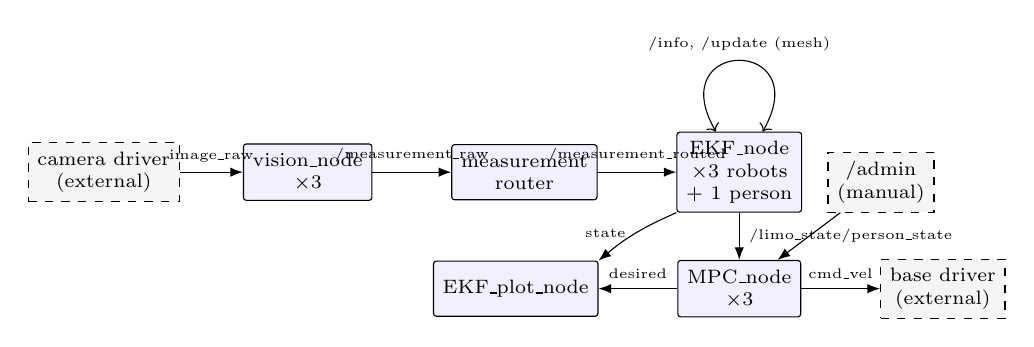
\begin{tikzpicture}[
  node distance=6mm and 8mm,
  box/.style={draw, rounded corners=1pt, align=center, minimum height=7mm, font=\scriptsize, fill=blue!6},
  ext/.style={draw, dashed, align=center, minimum height=7mm, font=\scriptsize, fill=gray!8},
  every path/.style={-{Latex[length=1.6mm]}, font=\tiny}
]
\node[ext] (cam) {camera driver\\(external)};
\node[box, right=of cam] (vis) {vision\_node\\$\times 3$};
\node[box, right=of vis, xshift=2mm] (rout) {measurement\\router};
\node[box, right=of rout, xshift=2mm] (ekf) {EKF\_node\\$\times 3$ robots\\$+\ 1$ person};
\node[box, below=of ekf] (mpc) {MPC\_node\\$\times 3$};
\node[ext, right=of mpc, xshift=2mm] (base) {base driver\\(external)};
\node[box, left=of mpc, xshift=-2mm] (plot) {EKF\_plot\_node};
\node[ext, above=of mpc, xshift=18mm] (admin) {/admin\\(manual)};

\draw (cam) -- node[above]{image\_raw} (vis);
\draw (vis) -- node[above]{/measurement\_raw} (rout);
\draw (rout) -- node[above]{/measurement\_routed} (ekf);
\draw (ekf) -- node[right]{/limo\_state\\/person\_state} (mpc);
\draw (mpc) -- node[above]{cmd\_vel} (base);
\draw (mpc.west) -- node[above]{desired} (plot.east);
\draw (ekf.south west) to[bend right=8] node[left]{state} (plot.north east);
\draw (admin) -- (mpc);

\draw[<->] (ekf) to[out=60, in=120, looseness=6] node[above, font=\tiny]{/info, /update (mesh)} (ekf);
\end{tikzpicture}
\caption{ROS~2 node/topic graph. Dashed boxes are external drivers (not part of this repository).
The four EKF\_node instances form a complete mesh over \texttt{/info} and \texttt{/update}: every
instance both publishes and subscribes, filtering messages by \texttt{id\_a}/\texttt{id\_b}.}
\label{fig:ros-graph}
\end{figure}

\begin{table}[t]
\centering
\caption{Custom ROS~2 messages (\texttt{project\_interfaces}).}
\label{tab:msgs}
\footnotesize
\begin{tabular}{@{}ll@{}}
\toprule
Message & Purpose \\
\midrule
\texttt{Measurement} & Relative pose $(x,y,\Delta\theta)$: $a$ observed $b$ \\
\texttt{Landmark} & IMDCL reply: $b$'s state, $\Phi_b$, $P_b$, addressed to $a$ \\
\texttt{Update} & Broadcast $\Gamma_a,\Gamma_b,W_1,W_2$ correction terms \\
\texttt{State} & Fused pose estimate, broadcast at $10\,\mathrm{Hz}$ \\
\texttt{Desired} & The three computed formation slot positions \\
\texttt{MPCprediction} & Predicted trajectory over the horizon (unused, Sec.~\ref{sec:problems}) \\
\bottomrule
\end{tabular}
\end{table}

\section{Results}
\label{sec:results}

Unlike a large synthetic sweep, what is available here is per-step logging (state, standard
deviation, $\mathrm{tr}(P)$, $\mathrm{tr}(\Phi)$, and, at every correction, the residual and
correction norm) written directly by \texttt{EKF\_node} during an actual run on the robots: three
robots with real wheel odometry feeding the predict step, and \texttt{sim\_vision\_node} injecting
structured, schema-compatible but synthetic relative measurements (uniform noise on a slowly
drifting target) in place of the camera pipeline, used to validate the estimator end to end on
hardware before wiring in live ArUco detections. The run spans $79.7\,\mathrm{s}$ at the nominal
$10\,\mathrm{Hz}$ filter rate, with a modest fraction of steps ($11$--$20\,\%$ across the three
robots) falling back to the zero-velocity filler prediction whenever a fresh odometry callback had
not arrived in time. \emph{Because the formation controller was not the object of this particular
log, the results below characterize the estimator's behaviour, not closed-loop formation
tracking.}

\subsection{Sensitivity to initial conditions}

Fig.~\ref{fig:trace-p} plots $\mathrm{tr}(P_i)$ for the three robots and the person over the run,
on a log scale. The three robots start at the identical prior $\mathrm{tr}(P)=0.300$
($P_0=0.1\,I_3$) and shrink monotonically to $0.090$--$0.107$ as cooperative corrections accumulate
-- a $\sim\!3\times$ reduction in $79.7\,\mathrm{s}$, driven by $592$ Update messages that every
agent applies identically over the run.

\begin{figure}[t]
\centering
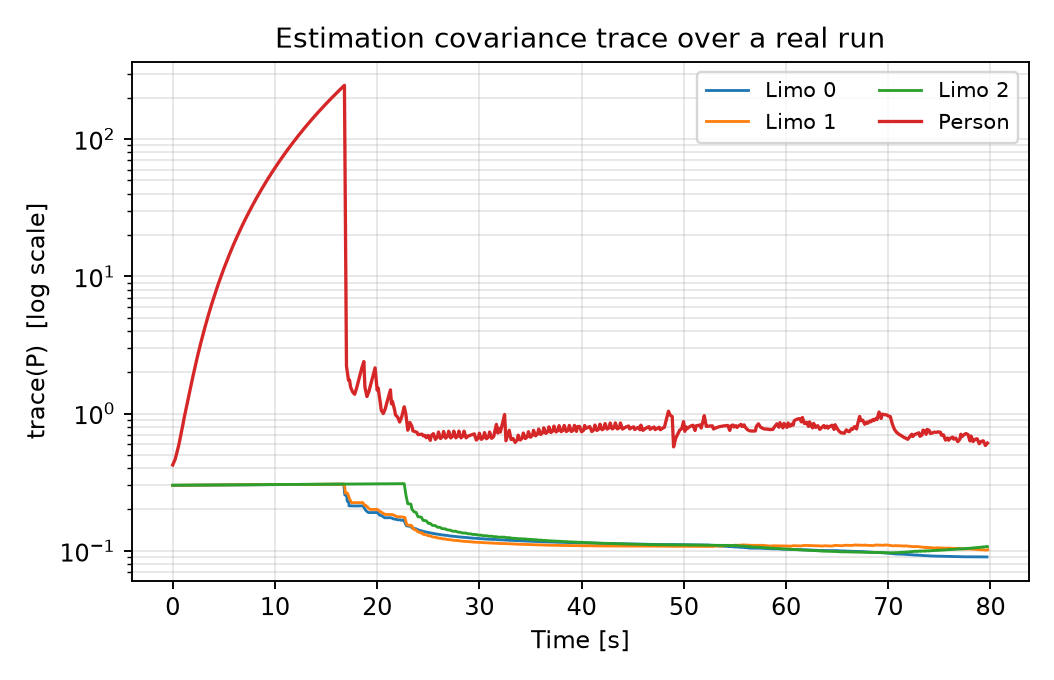
\includegraphics[width=\linewidth]{figures/trace-P.png}
\caption{$\mathrm{tr}(P)$ over a real run, log scale. The three robots converge smoothly; the
person's covariance ramps up unchecked for the first $\sim\!17\,\mathrm{s}$, then collapses by
more than two orders of magnitude the instant it is first directly observed.}
\label{fig:trace-p}
\end{figure}

The person tells a different story, and one directly attributable to how a small, confident
prior behaves once it is left unconstrained. $P_{0,p}=0.1\,I_4$ (\texttt{P0\_p} in
\texttt{conf\_limo.py}, the same $0.1\,I$ scale used for the robots' \texttt{P0\_rr}) is a
reasonable prior for a position estimate but says nothing informative about the velocity
sub-block $(v_x,v_y)$, which no sensor measures directly and which starts, like the rest of the
state, at $0$. In this run the round-robin measurement schedule happens to service two
robot-robot pairs before the person is first observed, so for the opening
$16.8\,\mathrm{s}$ the person's filter only ever predicts: $\mathrm{tr}(P)$ climbs
unchecked through $Q_p$ from $0.422$ to a peak of $246.7$, the unobserved velocity sub-block
inflating fastest because nothing bounds it. The very next correction that actually measures the
person collapses $\mathrm{tr}(P)$ from $246.7$ to $2.12$ in a single update -- a $\sim\!116\times$
drop -- confirming the filter is well-conditioned the instant it receives information; it is only
the \emph{absence} of information, not the algebra of the update itself, that let the covariance
run away. Over the remaining $63\,\mathrm{s}$ ($380$ further corrections in which the person is
the directly-measured agent, interleaved with corrections it only applies as a bystander) the
visible sawtooth in Fig.~\ref{fig:trace-p} is this same effect at smaller scale: every stretch
serviced only by robot-robot pairs lets $Q_p$ re-inflate the person's covariance a little before
the next direct correction pulls it back down, settling to $0.531$--$0.609$ by the end of the run.
The general lesson for this class of decentralized filter is that the initial covariance of a
state with \emph{no} direct sensor and \emph{no} self-generated prediction input (unlike the
robots, which at least integrate their own odometry every step) cannot be judged from its
magnitude alone: $P_{0,p}$ looks identical to the robots' prior on paper, but it is far more
exposed, because nothing caps how far it drifts before the first correction arrives, and how long
that takes is itself an accident of measurement scheduling rather than of the filter's design.

\subsection{How well it works, and problems}
\label{sec:problems}

\paragraph{What works.} The cooperative bookkeeping behaves as designed: all four agents log
exactly the same number of applied corrections ($592$), which is the basic consistency invariant
IMDCL is supposed to guarantee -- every agent, whether or not it was party to a given measurement,
ends up applying the identical correction to its local state of the world. Robot correction norms
settle to a median of $\sim\!2\,\mathrm{mm}$ per update after the initial transient
(Fig.~\ref{fig:correction-norm}), consistent with a converged, well-conditioned filter rather than
one chasing noise. \texttt{measurement\_router}'s per-pair outlier gate (rejecting a new sample
more than $0.5$ away from the currently buffered one on any axis) is a simple but effective guard
against a single corrupted detection propagating into the interim-master exchange.

\begin{figure}[t]
\centering
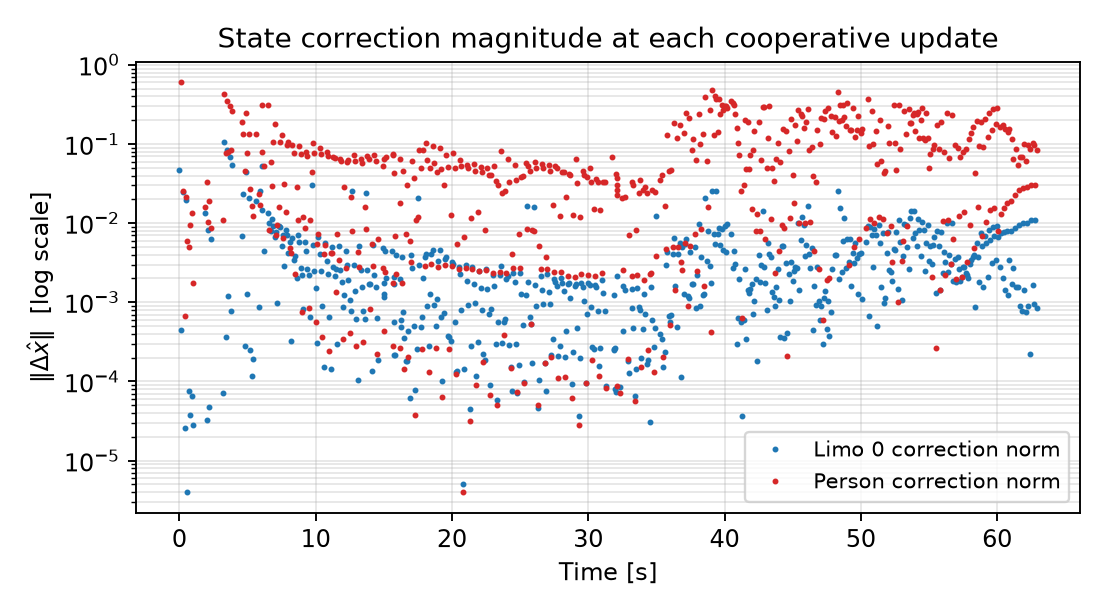
\includegraphics[width=\linewidth]{figures/correction-norm.png}
\caption{Correction magnitude at each applied update. The person (no self-prediction) sees
corrections roughly an order of magnitude larger than the robots throughout the run.}
\label{fig:correction-norm}
\end{figure}

\paragraph{Concrete problems found while building this report.} Cross-checking the running code
against its own documentation and against itself surfaced several issues that a purely
descriptive account of the intended design would not:
\begin{itemize}
\item \textbf{A silent formation-controller bug.} In
\texttt{MPC\_node.limo\_states\_callback}, the branch that is supposed to update the cached
position of the second teammate reads \texttt{self.limo\_2 == val} -- a comparison, not an
assignment. Every robot's belief about that particular teammate's position is therefore frozen at
its mission-start value for the entire run: both the Hungarian slot assignment
(Sec.~\ref{sec:desired-position}) and one of the two MPC collision-avoidance constraints
(Sec.~\ref{sec:control}) silently operate on a stale position instead of the live one. This does
not crash anything -- \texttt{==} is valid Python -- which is exactly why it is the kind of defect
that survives into a running system undetected.
\item \textbf{A dead prediction topic.} \texttt{MPC\_node} creates a publisher for
\texttt{mpc\_prediction} and \texttt{EKF\_plot\_node} subscribes to it, but the
\texttt{.publish()} call is commented out, so the visualizer's predicted-trajectory overlay is
permanently empty.
\item \textbf{A stale console-script entry.} \texttt{limo\_control/setup.py} still registers an
\texttt{EKF\_node} executable that no longer exists in that package (it moved to
\texttt{localization}); \texttt{ros2 run limo\_control EKF\_node} fails.
\item \textbf{Non-interchangeable simulation stand-ins.} Of the four nodes in the
\texttt{simulation} package, only \texttt{sim\_vision\_node} and \texttt{sim\_EKF\_node} are true
drop-in replacements (same topic name and type); \texttt{sim\_camera\_node} publishes on a fixed,
non-namespaced topic that \texttt{vision\_node} never subscribes to, and
\texttt{sim\_odometry\_node} publishes \texttt{std\_msgs/Float64MultiArray} where
\texttt{EKF\_node} expects \texttt{nav\_msgs/Odometry}.
\item \textbf{Two README/code divergences} beyond the YOLO point already discussed in
Sec.~\ref{sec:vision-node}: the estimator is described as an ``Interacting Multiple Model''
framework, but no IMM/multiple-model logic exists anywhere in \texttt{localization\_system.py} --
the code's own docstring correctly names it IMDCL; and deployment notes elsewhere in the
repository reference \texttt{'start\_ekf'}/\texttt{'stop\_ekf'} \texttt{/admin} commands that
\texttt{EKF\_node} never subscribes to (Sec.~\ref{sec:control}).
\end{itemize}
None of these are fatal to the estimator's core behaviour, which is exactly why they are worth
recording explicitly: a report written only from the intended design, rather than from the code
and its logs, would not have found any of them.

\section{Conclusion}
\label{sec:conclusion}

We implemented and ran, on a real three-robot LIMO fleet, a fully distributed cooperative
tracking system combining ArUco-based relative perception, an IMDCL cooperative filter that
reproduces a centralized EKF's estimate without ever exchanging the full joint covariance, and a
per-robot MPC that resolves formation-slot assignment locally through a shared deterministic
Hungarian solve. Logged data from a real run shows the filter converging as expected for the
robots and exposes a sharp, well-explained covariance transient for the person, whose state has no
direct sensor of its own -- a concrete demonstration of why the initial covariance of an
unobserved state block deserves separate tuning in this class of system. Writing this report
against the running code rather than against its design intent also surfaced several
implementation defects, most notably a silently no-op teammate-position update that undermines
both formation-slot assignment and one collision constraint, none of which are visible from the
algorithm description alone.

The most direct next steps are: fixing the identified formation-controller bug and re-evaluating
formation-tracking accuracy with it corrected; closing the loop with the live ArUco vision
pipeline instead of the synthetic measurement source used for the run analyzed here, and
re-running the same covariance analysis on that fully-hardware log; profiling MPC solve time on
the robots' onboard computer to confirm the $10$-iteration warm start keeps every step within the
$100\,\mathrm{ms}$ control period; and, more structurally, replacing the by-hand, per-node CLI
startup with proper ROS~2 launch files as the fleet size grows beyond three robots.

\begin{thebibliography}{9}

\bibitem{kia2016}
S.~S. Kia, S.~Rounds, and S.~Mart{\'i}nez, ``Cooperative Localization for Mobile Agents: A
Recursive Decentralized Algorithm Based on Kalman-Filter Decentralization,'' \emph{IEEE Control
Systems Magazine}, vol.~36, no.~2, pp.~86--101, 2016.

\bibitem{aruco2014}
S.~Garrido-Jurado, R.~Mu{\~n}oz-Salinas, F.~J.~Madrid-Cuevas, and M.~J.~Mar{\'i}n-Jim{\'e}nez,
``Automatic generation and detection of highly reliable fiducial markers under occlusion,''
\emph{Pattern Recognition}, vol.~47, no.~6, pp.~2280--2292, 2014.

\bibitem{casadi2019}
J.~A.~E.~Andersson, J.~Gillis, G.~Horn, J.~B.~Rawlings, and M.~Diehl, ``CasADi -- A software
framework for nonlinear optimization and optimal control,'' \emph{Mathematical Programming
Computation}, vol.~11, no.~1, pp.~1--36, 2019.

\bibitem{wachter2006}
A.~W{\"a}chter and L.~T.~Biegler, ``On the implementation of an interior-point filter
line-search algorithm for large-scale nonlinear programming,'' \emph{Mathematical Programming},
vol.~106, no.~1, pp.~25--57, 2006.

\bibitem{kuhn1955}
H.~W.~Kuhn, ``The Hungarian method for the assignment problem,'' \emph{Naval Research Logistics
Quarterly}, vol.~2, no.~1--2, pp.~83--97, 1955.

\bibitem{renelli-zanolini-artva}
A.~Renelli and L.~Zanolini, ``Distributed Multi-Drone ARTVA Search \& Rescue in GPS-denied
conditions,'' Intelligent Distributed Systems course project, University of Trento.

\end{thebibliography}

\end{document}
